\section*{Appendix} \label{appendix}

\appendix

\section{Additional Tables} \label{appendix:tables}

\subsection{Condition balance --- Player A} \label{appendix:sum_stats}

\begin{table}[!htbp]
    \centering
    \caption{Condition balance --- Player~A}
    \label{tab:treatment_balance}
    \begin{tabular}{l|rrr}
                  Variable &  \textit{Punishment} &  \textit{No-Punishment} &  $p$-value \\ \hline
                           Age &  $39.026$ &  $37.877$ &  $0.552$ \\
                        Female &  $0.487$ &  $0.494$ &  $1.000$ \\
         Socio-economic status &  $5.179$ &  $5.321$ &  $0.564$ \\
                   Went to uni &  $0.575$ &  $0.556$ &  $0.928$ \\
              Technology score &  $2.087$ &  $2.284$ &  $0.322$ \\
           Leadership position &  $0.362$ &  $0.333$ &  $0.824$ \\
    \end{tabular}
    \begin{minipage}{0.95\textwidth}\footnotesize
    \textit{Note:} Mean values by condition for Player~A, with $p$-values from two-sided $t$-tests for continuous variables and Chi-squared tests for binary variables. \textit{Socio-economic status} is self-reported on a $1$--$10$ scale. \textit{Went to uni} indicates a university degree. \textit{Technology score} is constructed from weekly device usage, programming skills, cryptocurrency knowledge, technology use at work, and similar items. \textit{Leadership position} indicates self-reported management or supervisory experience.
    \end{minipage}
\end{table}


\subsection{Condition balance --- Player B} \label{appendix:sum_stats_B}

\begin{table}[!htbp]
    \centering
    \caption{Condition balance --- Player~B}
    \label{tab:treatment_balance_B}
    \begin{tabular}{l|rrr}
                  Variable &  \textit{Punishment} &  \textit{No-Punishment} &  $p$-value \\ \hline
                           Age &  $37.087$ &  $42.356$ &  $0.011$ \\
                        Female &  $0.588$ &  $0.493$ &  $0.314$ \\
         Socio-economic status &  $5.425$ &  $5.110$ &  $0.204$ \\
                   Went to uni &  $0.688$ &  $0.481$ &  $0.013$ \\
              Technology score &  $1.363$ &  $1.333$ &  $0.869$ \\
           Leadership position &  $0.287$ &  $0.321$ &  $0.771$ \\
    \end{tabular}
    \begin{minipage}{0.95\textwidth}\footnotesize
    \textit{Note:} Mean values by condition for Player~B, with $p$-values from two-sided $t$-tests for continuous variables and Chi-squared tests for binary variables. \textit{Socio-economic status} is self-reported on a $1$--$10$ scale; \textit{Went to uni} indicates a university degree; \textit{Technology score} is constructed from weekly device usage, programming skills, cryptocurrency knowledge, technology use at work, and similar items; \textit{Leadership position} indicates self-reported management or supervisory experience.
    \end{minipage}
\end{table}


\subsection{Full regression results --- delegation decision} \label{appendix:regs}

\begin{table}[!htbp]
\centering
\caption{Determinants of the delegation decision --- full controls}
\label{tab:reg_delegation}
\begin{tabular}{@{\extracolsep{5pt}}lcc|c}
\\[-1.8ex]\hline
\hline \\[-1.8ex]
& \multicolumn{3}{c}{Dependent variable: \textit{Delegation}}\\[0.1cm]
& \multicolumn{2}{c}{\textit{Full sample}} & \textit{Punishment only} \\
\\[-1.8ex] & (1) & (2) & (3) \\
\hline \\[-1.8ex]
 No-Punishment indicator & $0.677$ & $0.757$ &  \\
  & $(0.320)$ & $(0.334)$ &  \\[0.1cm]
 Punishment beliefs: bad outcome &  &  & $0.937$ \\
  &  &  & $(0.751)$ \\[0.1cm]
 Punishment beliefs: good outcome &  &  & $1.579$ \\
  &  &  & $(0.741)$ \\[0.1cm]
 Task performance &  & $-0.192$ & $-0.609$ \\
  &  & $(0.128)$ & $(0.236)$ \\[0.1cm]
 Age &  & $-0.004$ & $0.064$ \\
  &  & $(0.015)$ & $(0.030)$ \\[0.1cm]
 Female &  & $0.350$ & $1.334$ \\
  &  & $(0.369)$ & $(0.793)$ \\[0.1cm]
 Socio-economic status &  & $-0.058$ & $-0.003$ \\
  &  & $(0.116)$ & $(0.219)$ \\[0.1cm]
 Went to uni &  & $0.091$ & $-0.433$ \\
  &  & $(0.364)$ & $(0.707)$ \\[0.1cm]
 Technology score &  & $-0.078$ & $0.059$ \\
  &  & $(0.153)$ & $(0.283)$ \\[0.1cm]
 Leadership position &  & $0.676$ & $-0.387$ \\
  &  & $(0.367)$ & $(0.729)$ \\[0.1cm]
 Constant & $-0.302$ & $0.402$ & $-1.842$ \\
  & $(0.226)$ & $(0.930)$ & $(2.103)$ \\[0.1cm]
\hline \\[-1.8ex]
 N & $161$ & $159$ & $60$ \\
 Pseudo $R^2$ & $0.020$ & $0.049$ & $0.246$ \\
\hline
\hline \\[-1.8ex]
\multicolumn{4}{p{0.85\textwidth}}{\footnotesize \textit{Note:} Logit estimates with robust (HC1) standard errors in parentheses. Two subjects in Column~(2) are dropped due to missing socio-demographic data. Column~(3) restricts to the \textit{Punishment} condition and excludes subjects who failed the attention check on the belief-elicitation screen, as preregistered. The belief variables in Column~(3) are within-subject differences in expected punishment between non-delegated and delegated decisions for each outcome. Following AEA editorial policy, significance stars are not reported in the table.}
\end{tabular}
\end{table}


\subsection{Robustness --- delegation decision} \label{appendix:reg_delegation_robustness}

\begin{table}[!htbp]
\centering
\scriptsize
\caption{Determinants of the delegation decision --- robustness}
\label{tab:reg_delegation_robustness}
\begin{tabular}{@{\extracolsep{5pt}}lcc|c}
\\[-1.8ex]\hline
\hline \\[-1.8ex]
& \multicolumn{3}{c}{Dependent variable: \textit{Delegation}}\\[0.1cm]
& \multicolumn{2}{c}{\textit{Full sample}} & \textit{Punishment} (no excl.) \\
\\[-1.8ex] & (1) & (2) & (3) \\
\hline \\[-1.8ex]
 Punishment indicator & $-0.771$ & $-0.677$ &  \\
  & $(0.336)$ & $(0.320)$ &  \\[0.1cm]
 Task performance & $-0.277$ &  & $-0.395$ \\
  & $(0.149)$ &  & $(0.185)$ \\[0.1cm]
 Overconfidence & $-0.103$ &  &  \\
  & $(0.094)$ &  &  \\[0.1cm]
 Punishment beliefs: bad outcome (no del.~$-$~del.) &  &  & $-0.277$ \\
  &  &  & $(0.499)$ \\[0.1cm]
 Punishment beliefs: good outcome (no del.~$-$~del.) &  &  & $0.812$ \\
  &  &  & $(0.529)$ \\[0.1cm]
\hline \\[-1.8ex]
 Controls & yes & no & yes \\
 Attention-check excl. & yes (Player A) & n/a & no \\
 Sample & Full & Full & Punishment \\
 N & $159$ & $161$ & $78$ \\
 Pseudo $R^2$ & $0.055$ & $0.020$ & $0.114$ \\
\hline
\hline \\[-1.8ex]
\multicolumn{4}{p{0.85\textwidth}}{\footnotesize \textit{Note:} Robustness specifications for the delegation logit. Column (1) adds \textit{overconfidence} (defined as the weighted-average belief about own performance minus actual performance) to the main full-sample specification. The treatment effect remains: \textit{Punishment indicator} $p=0.022$. \textit{Overconfidence} is not significantly associated with delegation $p=0.272$. Column (2) reproduces the unconditional treatment effect for completeness ($p=0.034$; identical to the main Col (1)). Column (3) restricts to the \textit{Punishment} condition and includes the within-subject belief differences but \textit{does not} exclude subjects who failed the belief-screen attention check; the heterogeneity result is preserved: \textit{Task performance} $p=0.033$; \textit{Punishment beliefs: good outcome} $p=0.125$. Robust HC1 standard errors in parentheses. Following AEA editorial policy, significance stars are not reported in the table.}
\end{tabular}
\end{table}


\subsection{Determinants of Player~B's chosen punishment} \label{appendix:reg_punishment}

\begin{table}[!htbp]
\centering
\caption{Determinants of Player~B's chosen punishment}
\label{tab:reg_punishment}
\begin{tabular}{@{\extracolsep{5pt}}lccc|ccc}
\\[-1.8ex]\hline
\hline \\[-1.8ex]
& \multicolumn{6}{c}{Dependent variable: \textit{Punishment}}\\[0.1cm]
& \multicolumn{3}{c}{\textit{Full sample}} & \multicolumn{3}{c}{\textit{Passers}} \\
& \textit{Level} (\pounds) & \multicolumn{2}{c}{\textit{Difference} (\pounds)} & \textit{Level} (\pounds) & \multicolumn{2}{c}{\textit{Difference} (\pounds)} \\
\\[-1.8ex] & (1) & (2) & (3) & (4) & (5) & (6) \\
\hline \\[-1.8ex]
 Delegated & $0.032$ &  &  & $0.001$ &  &  \\
  & $(0.052)$ &  &  & $(0.054)$ &  &  \\[0.1cm]
 Bad outcome & $0.256^{***}$ & $0.103^{*}$ & $0.103^{*}$ & $0.260^{***}$ & $0.078$ & $0.078$ \\
  & $(0.071)$ & $(0.057)$ & $(0.059)$ & $(0.080)$ & $(0.052)$ & $(0.053)$ \\[0.1cm]
 Delegated $\times$ Bad outcome & $-0.103^{*}$ &  &  & $-0.078$ &  &  \\
  & $(0.058)$ &  &  & $(0.052)$ &  &  \\[0.1cm]
 Player B belief about Player A perf. & $-0.020$ &  & $-0.006$ & $0.001$ &  & $-0.006$ \\
  & $(0.032)$ &  & $(0.029)$ & $(0.037)$ &  & $(0.038)$ \\[0.1cm]
 Age & $0.002$ &  & $-0.009^{**}$ & $-0.001$ &  & $-0.009^{**}$ \\
  & $(0.005)$ &  & $(0.003)$ & $(0.006)$ &  & $(0.004)$ \\[0.1cm]
 Female & $-0.100$ &  & $-0.012$ & $-0.064$ &  & $0.003$ \\
  & $(0.128)$ &  & $(0.109)$ & $(0.140)$ &  & $(0.132)$ \\[0.1cm]
 Socio-economic status & $0.083^{*}$ &  & $0.029$ & $0.072$ &  & $0.041$ \\
  & $(0.047)$ &  & $(0.024)$ & $(0.049)$ &  & $(0.028)$ \\[0.1cm]
 Went to uni & $-0.196$ &  & $0.051$ & $-0.098$ &  & $0.023$ \\
  & $(0.140)$ &  & $(0.070)$ & $(0.142)$ &  & $(0.075)$ \\[0.1cm]
 Technology score & $0.073$ &  & $-0.022$ & $0.030$ &  & $-0.012$ \\
  & $(0.053)$ &  & $(0.027)$ & $(0.059)$ &  & $(0.033)$ \\[0.1cm]
 Leadership position & $0.083$ &  & $0.143$ & $0.061$ &  & $0.174$ \\
  & $(0.142)$ &  & $(0.122)$ & $(0.164)$ &  & $(0.145)$ \\[0.1cm]
 Constant & $-0.077$ & $-0.032$ & $0.116$ & $0.020$ & $-0.001$ & $0.076$ \\
  & $(0.328)$ & $(0.051)$ & $(0.320)$ & $(0.374)$ & $(0.053)$ & $(0.397)$ \\[0.1cm]
\hline \\[-1.8ex]
 Observations & $320$ & $160$ & $160$ & $268$ & $134$ & $134$ \\
 Subjects & $80$ & $80$ & $80$ & $67$ & $67$ & $67$ \\
 Adj.\ $R^2$ & $0.077$ & $0.008$ & $0.038$ & $0.030$ & $0.001$ & $0.043$ \\
\hline
\hline \\[-1.8ex]
\multicolumn{7}{p{0.85\textwidth}}{\footnotesize \textit{Note:} Columns~(1) and~(4): OLS regression of Player~B's chosen punishment level on a delegation indicator, a bad-outcome indicator, their interaction, Player~B's belief about Player~A's performance, and a vector of socio-demographic controls; sample stacked over the four (delegation, outcome) cells of the strategy method (4 observations per Player~B). Columns~(2)/(5) and~(3)/(6): OLS regression of the within-subject delegation insulation (\textit{punish\_nodel} $-$ \textit{punish\_del}) on a bad-outcome indicator and, in Columns~(3)/(6), additional controls; sample stacked over the two outcome cells (2 observations per Player~B). In the difference specifications, the intercept is the average insulation in the good-outcome cell and the bad-outcome coefficient is the additional insulation in the bad-outcome cell. Columns~(1)--(3) use the full Punishment-condition sample. Columns~(4)--(6) restrict to Player~Bs who passed the attention check on the punishment-elicitation screen, as preregistered. Standard errors clustered at the Player~B level. Significance: $^{*}\,p<0.10$; $^{**}\,p<0.05$; $^{***}\,p<0.01$ (two-sided).}
\end{tabular}
\end{table}


\subsection{Robustness --- Player~B's chosen punishment} \label{appendix:reg_punishment_robustness}

\begin{table}[!htbp]
\centering
\caption{Determinants of Player~B's chosen punishment --- robustness}
\label{tab:reg_punishment_robustness}
\begin{tabular}{lcc}
\\[-1.8ex]\hline
\hline \\[-1.8ex]
& \multicolumn{2}{c}{Dependent variable: \textit{Punishment}}\\[0.1cm]
& \textit{Excl.} & \textit{Incl. att.\ failers} \\
\\[-1.8ex] & (1) & (2) \\
\hline \\[-1.8ex]
 Delegated & $0.001$ & $0.032$ \\
  & $(0.054)$ & $(0.052)$ \\[0.1cm]
 Bad outcome & $0.260$ & $0.256$ \\
  & $(0.080)$ & $(0.071)$ \\[0.1cm]
 Delegated $\times$ Bad outcome & $-0.078$ & $-0.103$ \\
  & $(0.052)$ & $(0.058)$ \\[0.1cm]
 Player B belief about Player A perf. (wa) & $0.001$ & $-0.020$ \\
  & $(0.037)$ & $(0.032)$ \\[0.1cm]
 Age & $-0.001$ & $0.002$ \\
  & $(0.006)$ & $(0.005)$ \\[0.1cm]
 Female & $-0.064$ & $-0.100$ \\
  & $(0.140)$ & $(0.128)$ \\[0.1cm]
 Socio-economic status & $0.072$ & $0.083$ \\
  & $(0.049)$ & $(0.047)$ \\[0.1cm]
 Went to uni & $-0.098$ & $-0.196$ \\
  & $(0.142)$ & $(0.140)$ \\[0.1cm]
 Technology score & $0.030$ & $0.073$ \\
  & $(0.059)$ & $(0.053)$ \\[0.1cm]
 Leadership position & $0.061$ & $0.083$ \\
  & $(0.164)$ & $(0.142)$ \\[0.1cm]
 Constant & $0.020$ & $-0.077$ \\
  & $(0.374)$ & $(0.328)$ \\[0.1cm]
\hline \\[-1.8ex]
 Attention-check excl. & yes & no \\
 N (subject-by-cell) & $268$ & $320$ \\
 Adj.\ $R^2$ & $0.030$ & $0.077$ \\
\hline
\hline \\[-1.8ex]
\multicolumn{3}{p{0.85\textwidth}}{\footnotesize \textit{Note:} Punishment regression with Player~B's belief about Player~A's performance (\textit{wa\_difficulty}) added as a regressor. Column (1) excludes Player~Bs who failed the punishment-screen attention check (preregistered); Column (2) keeps them. Standard errors clustered at the Player~B level. The delegation, outcome, and interaction coefficients are stable across both specifications, and the belief regressor is not significantly associated with chosen punishment. H2 paired-test on the bad-outcome cell: with exclusion paired-$t$ $p=0.153$, Wilcoxon $p=0.533$ ($n=67$); without exclusion paired-$t$ $p=0.131$, Wilcoxon $p=0.544$ ($n=80$). Following AEA editorial policy, significance stars are not reported.}
\end{tabular}
\end{table}


\section{Preregistration and deviations} \label{appendix:pap}

The experiment was preregistered prior to data collection. The preregistration document specifies the two hypotheses (H1 and H2 in the body), the sample-size target ($80$ subjects per role per condition, motivated by an ex-ante power calculation reproduced in the registry), the randomisation procedure, the attention-check exclusion rule, and the test direction for each preregistered comparison.

For full transparency, the table below summarises every analysis reported in the body of the paper, the corresponding preregistered specification, and any deviation. We treat the H1 reversal in Section~\ref{sec:result1} as a confirmatory test of the preregistered direction (which it rejects), and all subsequent mechanism analyses (Section~\ref{sec:mechanism}) as exploratory.

\begin{table}[!htbp]
\centering
\caption{Preregistered tests, reported tests, and deviations}
\label{tab:pap_deviations}
\begin{tabular}{p{0.32\textwidth}|p{0.32\textwidth}|p{0.30\textwidth}}
\hline
\hline
Preregistered specification & As reported & Deviation / rationale \\ \hline
H1: between-subject test of \textit{Punishment} vs \textit{No-Punishment} delegation rates; one-sided in the H1 direction (more delegation under \textit{Punishment}) & Two-sided Chi-squared and Fisher's exact, $p=0.049$ / $0.041$ & Direction reversed; one-sided test in H1 direction is non-significant by construction. We report two-sided to be transparent about what the data show. \\[0.3cm]
H2: paired test of Player~B punishment in the bad-outcome cell, delegated vs non-delegated, attention-check passers only & Paired $t$-test, $p=0.153$; Wilcoxon signed-rank, $p=0.533$ & As preregistered. \\[0.3cm]
Logit of delegation on condition + controls (Table~\ref{tab:del_decision_determinants}, Cols (1)--(2)) & As reported & As preregistered. \\[0.3cm]
Logit on \textit{Punishment} sub-sample with belief differences (Col (3)) & As reported & Specification preregistered; sample restriction follows the preregistered attention-check rule. \\[0.3cm]
Mechanism analyses M1--M4 (Section~\ref{sec:mechanism}) & As reported & \textit{Not preregistered.} Treated as exploratory throughout. \\[0.3cm]
Effort-comparison statistics among non-delegators (Section~\ref{sec:mechanism}, M2) & As reported & \textit{Not preregistered.} Treated as exploratory. \\
\hline
\hline
\multicolumn{3}{p{0.95\textwidth}}{\footnotesize \textit{Note:} The preregistration document is available at \textit{[registry link to be added at submission]}. The registry ID is \textit{[ID to be added at submission]}.}
\end{tabular}
\end{table}

\section{CONSORT-style flow diagram} \label{appendix:attrition}

A CONSORT-style flow diagram showing recruitment, attrition, attention-check exclusion, and final analysis sample size by condition and role is in preparation and will appear here once the analysis pipeline produces the underlying counts. The structure of the diagram is sketched below; cell counts pending.

\begin{figure}[!htbp]
\centering
\caption{Flow of participants through the experiment --- structure (counts pending)}
\label{fig:consort}
\begin{tikzpicture}[node distance=0.6cm and 0.6cm, every node/.style={draw, rectangle, align=center, font=\footnotesize, inner sep=4pt}]
\node (rand) {Completed experiment ($N=322$)\\Recruitment-funnel counts (invited / consented) pending Prolific audit log};
\node (pun) [below left=of rand, xshift=-0.4cm] {\textit{Punishment} condition\\Player A: $80$\\Player B: $80$};
\node (nopun) [below right=of rand, xshift=0.4cm] {\textit{No-Punishment} condition\\Player A: $81$\\Player B: $81$};
\node (att_p) [below=of pun] {Attention-check exclusion\\Player A: $19$\\Player B: $13$};
\node (att_np) [below=of nopun] {Attention-check exclusion\\Player A: $11$\\Player B: $13$};
\node (final_p) [below=of att_p] {Analysis sample\\Player A: $61$\\Player B: $67$};
\node (final_np) [below=of att_np] {Analysis sample\\Player A: $70$\\Player B: $68$};
\draw[->] (rand) -- (pun);
\draw[->] (rand) -- (nopun);
\draw[->] (pun) -- (att_p);
\draw[->] (nopun) -- (att_np);
\draw[->] (att_p) -- (final_p);
\draw[->] (att_np) -- (final_np);
\end{tikzpicture}
\end{figure}

\section{Additional Figures} \label{appendix:figures}

\subsection{Experimental timelines}

\begin{figure}[!htbp]
    \centering
    \caption{Experimental timeline --- Player A}
    \label{fig:design_playerA}
    \scalebox{0.85}{
    \begin{tikzpicture}[node distance=0.55cm and 0.4cm, every node/.style={draw, rectangle, align=center, font=\scriptsize, minimum width=2.4cm, minimum height=0.7cm, inner sep=2pt}, ac/.style={fill=red!15}]
    \node (consent) {Consent};
    \node (rounds) [right=of consent] {10 prediction\\rounds (incentivised)};
    \node (match) [right=of rounds] {Matching\\with Player B};
    \node (deleg) [below=of match] {Delegation\\decision};
    \node (predict) [below=of deleg] {(if not delegated)\\11th prediction\\\& confidence};
    \node (beliefs) [left=of predict, ac] {Beliefs about\\punishment\\\textit{(attention check)}};
    \node (selfperf) [left=of beliefs] {Self-performance\\assessment};
    \node (popperf) [below=of selfperf] {Population-performance\\assessment};
    \node (risk) [right=of popperf] {Risk preferences\\(MPL)};
    \node (qx) [right=of risk] {Questionnaire};
    \node (payoff) [right=of qx] {Payoff};
    \draw[->] (consent) -- (rounds);
    \draw[->] (rounds) -- (match);
    \draw[->] (match) -- (deleg);
    \draw[->] (deleg) -- (predict);
    \draw[->] (predict) -- (beliefs);
    \draw[->] (beliefs) -- (selfperf);
    \draw[->] (selfperf) -- (popperf);
    \draw[->] (popperf) -- (risk);
    \draw[->] (risk) -- (qx);
    \draw[->] (qx) -- (payoff);
    \end{tikzpicture}
    }
    \begin{minipage}{0.95\linewidth}
    \footnotesize
    \textit{Note:} Screen sequence presented to Player~A. The shaded screen carries the preregistered attention check used to identify subjects excluded from belief-related analyses. The 11th-prediction-and-confidence screen is skipped if Player~A delegates to the algorithm.
    \end{minipage}
\end{figure}

\begin{figure}[!htbp]
    \centering
    \caption{Experimental timeline --- Player B}
    \label{fig:design_playerB}
    \scalebox{0.85}{
    \begin{tikzpicture}[node distance=0.55cm and 0.5cm, every node/.style={draw, rectangle, align=center, font=\scriptsize, minimum width=2.7cm, minimum height=0.8cm, inner sep=2pt}, ac/.style={fill=red!15}]
    \node (consent) {Consent};
    \node (match) [right=of consent] {Matching with Player A\\\& task description};
    \node (pun) [right=of match, ac] {Punishment elicitation\\(\textit{Punishment} cond.)\\or hypothetical-punishment\\(\textit{No-Punishment} cond.)\\\textit{(attention check)}};
    \node (diff) [below=of pun] {Task-difficulty\\perception};
    \node (risk) [left=of diff] {Risk preferences\\(MPL)};
    \node (qx) [left=of risk] {Questionnaire};
    \node (payoff) [below=of qx] {Payoff};
    \draw[->] (consent) -- (match);
    \draw[->] (match) -- (pun);
    \draw[->] (pun) -- (diff);
    \draw[->] (diff) -- (risk);
    \draw[->] (risk) -- (qx);
    \draw[->] (qx) -- (payoff);
    \end{tikzpicture}
    }
    \begin{minipage}{0.95\linewidth}
    \footnotesize
    \textit{Note:} Screen sequence presented to Player~B. The shaded screen carries the preregistered attention check used to identify subjects excluded from punishment-related analyses. In the \textit{No-Punishment} condition, no actual punishment is implemented; the elicitation is hypothetical and serves to maintain comparability of the screen sequence across conditions.
    \end{minipage}
\end{figure}

\subsection{Punishment frequencies} \label{appendix:figs:punishment}

\begin{figure}[!htbp]
    \centering
    \caption{Frequencies of punishment and beliefs about punishment}
    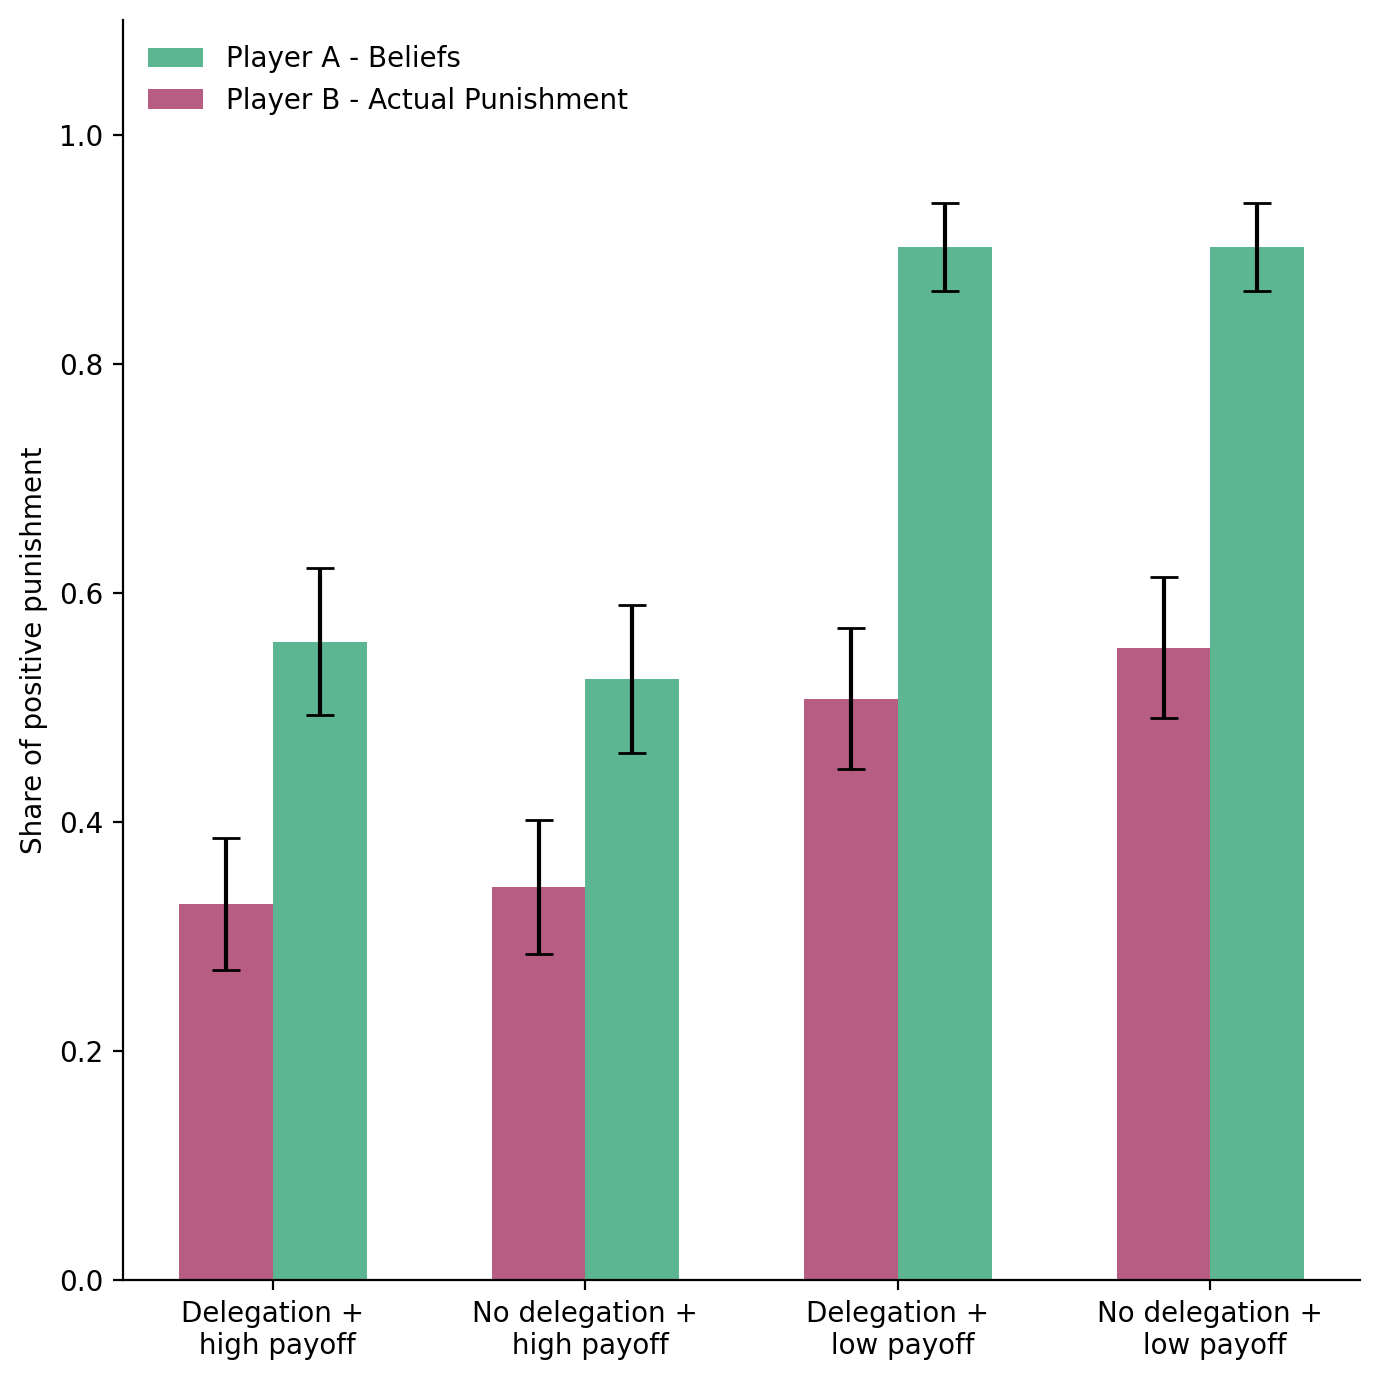
\includegraphics[width=0.6\linewidth]{figures/punishment_shares.png}
    \label{fig:punishment_frequencies}
    \begin{minipage}{0.85\linewidth}
    \footnotesize
    \textit{Note:} Share of Player~Bs choosing strictly positive punishment in each of the four scenarios (solid bars) and share of Player~As assigning a strictly positive expected punishment in each scenario (hollow bars).
    \end{minipage}
\end{figure}
